\begin{dang}{~}
	\begin{enumerate}[1]
		\item Điều kiện hàm ẩn có dạng $A(x)f(x)+B(x)f'(x)=h(x)$.\quad $(1)$\\
		Ý tưởng giải.
		\begin{itemize}
			\item Ta cần nhân thêm một lượng $u(x)$ vào  $(1)$ để tạo thành \break $u'(x) f(x)+u(x) f'(x)=u(x) \cdot h(x)$ và lúc này.
			\begin{align*}
				&\, u'(x) f(x)+u(x) f'(x)=u(x) \cdot h(x) \\
				\Leftrightarrow&\,\left[u(x) f(x)\right]'=u(x) \cdot h(x) \\
				\Rightarrow&\, \displaystyle\int\left[u(x) f(x)\right] \mathrm{\,d} x=\displaystyle\int u(x) \cdot h(x) d x \\
				\Rightarrow&\, u(x) f(x)=\displaystyle\int u(x) \cdot h(x) \mathrm{\,d} x \\
				\Rightarrow&\, f(x)=\dfrac{\displaystyle\int u(x) \cdot h(x) \mathrm{\,d} x}{u(x)}
			\end{align*}
			\item Cách tìm $u(x)$.\\
			$u(x)$ được chọn sao cho  $\heva{&u'(x)=A(x) \\ &u(x)=B(x).}$\\
			Suy ra 
			\begin{align*}
				&\,\dfrac{u'(x)}{u(x)}=\dfrac{A(x)}{B(x)}\\
				\Rightarrow&\, \displaystyle\int \dfrac{u'(x)}{u(x)} \mathrm{\,d} x=\displaystyle\int \dfrac{A(x)}{B(x)} \mathrm{\,d} x\\
				\Rightarrow&\, \ln |u(x)|=\displaystyle\int \dfrac{A(x)}{B(x)} \mathrm{\,d} x\\
				\Rightarrow&\, u(x)=\mathrm{e}^{\displaystyle\int\tfrac{A(x)}{B(x)}} \mathrm{\,d} x
			\end{align*}
		\end{itemize}
		Tóm lại phương pháp giải $A(x)f(x)+B(x)f'(x)=h(x)$\quad $(1)$ như sau.
		\begin{itemize}
			\item \textbf{Bước 1.} Tìm $u(x)$. $u(x)=\mathrm{e}^{\displaystyle\int\tfrac{A(x)}{B(x)}} \mathrm{\,d} x$.
			\item \textbf{Bước 2.} Nhân $u(x)$ vào $(1)$ suy ra $f(x)=\dfrac{\displaystyle\int\limits u(x) \cdot h(x) \mathrm{\,d}x}{u(x)}$.
		\end{itemize}
		\item Một số dạng đặc biệt của $(1)$.
		\begin{enumerate}
			\item Điều kiện hàm ẩn có dạng $\hoac{&f'(x)+f(x)=h(x)\\ &f'(x)-f(x)=h(x).}$\\
			Phương pháp giải.
			\begin{itemize}
				\item $f'(x)+f(x)=h(x)$.\\
				Nhân hai vế với $\mathrm{e}^x$ ta được $$\mathrm{e}^x \cdot f'(x)+\mathrm{e}^x \cdot f(x)=\mathrm{e}^x \cdot h(x) \Leftrightarrow\left[\mathrm{e}^x \cdot f(x)\right]'=\mathrm{e}^x \cdot h(x).$$
				Suy ra $\mathrm{e}^x \cdot f(x)=\displaystyle\int \mathrm{e}^x \cdot h(x)  \mathrm{\,d} x$.\\
				Từ đây ta dễ dàng tính được $f(x)$.
				\item $f'(x)-f(x)=h(x)$.\\
				Nhân hai vế với $\mathrm{e}^{-x}$ ta được $$\mathrm{e}^{-x} \cdot f'(x)-\mathrm{e}^{-x} \cdot f(x)=\mathrm{e}^{-x} \cdot h(x) \Leftrightarrow\left[\mathrm{e}^{-x} \cdot f(x)\right]'=\mathrm{e}^{-x} \cdot h(x).$$
				Suy ra $\mathrm{e}^{-x} \cdot f(x)=\displaystyle\int \mathrm{e}^{-x} \cdot h(x)  \mathrm{\,d} x$.\\
				Từ đây ta dễ dàng tính được $f(x)$.
			\end{itemize}
			\item Điều kiện hàm ẩn có dạng $f'(x)+p(x)\cdot f(x)=h(x)$.\\
			\textbf{Phương pháp giải.}\\
			Nhân hai vế với $\mathrm{e}^{\displaystyle\int\limits p(x) \mathrm{\,d} x}$ ta được
			\begin{align*}
				&\,f'(x) \cdot \mathrm{e}^{\displaystyle\int\limits p(x) \mathrm{\,d} x}+p(x) \cdot \mathrm{e}^{\displaystyle\int\limits p(x) \mathrm{\,d} x} \cdot f(x)=h(x) \cdot \mathrm{e}^{\displaystyle\int\limits p(x) \mathrm{\,d}x}\\
				\Leftrightarrow&\, \left[f(x) \cdot \mathrm{e}^{\displaystyle\int\limits p(x) \mathrm{\,d} x}\right]'=h(x) \cdot \mathrm{e}^{\displaystyle\int\limits p(x) \mathrm{\,d} x}.
			\end{align*}
			Suy ra $f(x) \cdot e^{\displaystyle\int p(x)\mathrm{\,d} x}=\displaystyle\int \mathrm{e}^{\displaystyle\int\limits p(x) \mathrm{e} x} h(x)  \mathrm{\,d} x$.\\
			Từ đây ta dễ dàng tính được $f(x)$.
		\end{enumerate}
	\end{enumerate}	
\end{dang}
\TN
\Opensolutionfile{ans}[ans/ans-LC-2-C4B1CD3.1]
\begin{ex}%[2D4V1-4]
	Cho hàm số $f(x)$ thỏa mãn $f(x)+f'(x)= \mathrm{e}^{-x}$, $\forall x \in \mathbb{R}$ và $f(0)=2$. Tất cả các nguyên hàm của $f(x)\mathrm{e}^x$ là
	\choice
	{$x^2+x+C$}
	{$2 x^2+2 x+C$}
	{$2 x^2+x+C$}
	{\True $\dfrac{1}{2} x^2+2 x+C$}
	\loigiai{
		Ta có \begin{align*}
			f(x)+f'(x)= \mathrm{e}^{-x}
			&\, \Leftrightarrow f(x)  \mathrm{e}^x+f'(x)  \mathrm{e}^x=1 \\
			&\, \Leftrightarrow\left(f(x)  \mathrm{e}^x\right)'=1 \\
			&\, \Rightarrow f(x)  \mathrm{e}^x=\displaystyle\int x \mathrm{\,d} x \\
			&\, \Leftrightarrow f(x)  \mathrm{e}^x=x+C.
		\end{align*}
		Vì $f(0)=2$ nên $ C=2$.\\
		Suy ra $f(x)  \mathrm{e}^x=x+2
		\Rightarrow \displaystyle\int f(x)  \mathrm{e}^x d x=\displaystyle\int(x+2) \mathrm{\,d} x=\dfrac{1}{2} x^2+2 x+C$.
	}
\end{ex}

\begin{ex}%[2D4V1-4]
	Cho hàm số $y=f(x)$ liên tục trên $\mathbb{R}$ thỏa mãn $f'(x)+2 x \cdot f(x)= \mathrm{e}^{-x^2}$, $\forall x \in \mathbb{R}$ và $f(0)=0$. Tính $f(1)$.
	\choice
	{$f(1)= \mathrm{e}^2$}
	{$f(1)=-\dfrac{1}{ \mathrm{e}}$}
	{$f(1)=\dfrac{1}{ \mathrm{e}^2}$}
	{\True $f(1)=\dfrac{1}{ \mathrm{e}}$}
	\loigiai{
		Ta có
		\begin{align*}
			&\, f'(x)+2 x \cdot f(x)= \mathrm{e}^{-x^2} \\
			\Leftrightarrow&\,  \mathrm{e}^{x^2} f'(x)+2 x \cdot  \mathrm{e}^{x^2} \cdot f(x)=1 \\
			\Leftrightarrow&\,\left( \mathrm{e}^{x^2} \cdot f(x)\right)'=1\\
			\Rightarrow&\,\displaystyle\int\left(\mathrm{e}^{x^2} \cdot f(x)\right)' \mathrm{\,d} x=\displaystyle\int \mathrm{\,d} x\\
			\Rightarrow&\,  \mathrm{e}^{x^2} \cdot f(x)=x+C \\
			\Rightarrow&\, f(x)=\dfrac{x+C}{\mathrm{e}^{x^2}}.
		\end{align*}
		Vì $f(0)=0 \Rightarrow C=0$.\\
		Do đó $f(x)=\dfrac{x}{ \mathrm{e}^{x^2}}$.\\
		Vậy $f(1)=\dfrac{1}{ \mathrm{e}}$.
	}
\end{ex}

\begin{ex}%[2D4V1-2]
	Cho hàm số $y=f(x)$ liên tục trên $\mathbb{R} \setminus \{-1 ; 0\}$ thỏa mãn điều kiện $f(1)=-2 \ln 2$ và $x \cdot(x+1) \cdot f'(x)+f(x)=x^2+x$. Biết $f(2)=a+b \cdot \ln 3$  ($a$, $b \in \mathbb{Q}$). Giá trị $2\left(a^2+b^2\right)$ là
	\choice
	{$\dfrac{27}{4}$}
	{\True  $9$}
	{$\dfrac{3}{4}$}
	{$\dfrac{9}{2}$}
	\loigiai{
		Chia cả hai vế của biểu thức $x \cdot(x+1) \cdot f'(x)+f(x)=x^2+x$ cho $(x+1)^2$ ta có
		$$ \dfrac{x}{x+1} \cdot f'(x)+\dfrac{1}{(x+1)^2} f(x)=\dfrac{x}{x+1} \\
		\Leftrightarrow\left[\dfrac{x}{x+1} \cdot f(x)\right]'=\dfrac{x}{x+1}.$$
		Do đó $$\dfrac{x}{x+1} \cdot f(x)=\displaystyle\int\limits\left[\dfrac{x}{x+1} \cdot f(x)\right]'  \mathrm{\,d} x=\displaystyle\int\limits \dfrac{x}{x+1} \mathrm{\,d} x=\displaystyle\int\limits\left(1-\dfrac{1}{x+1}\right)  \mathrm{\,d} x=x-\ln |x+1|+C.$$
		Do $f(1)=-2 \ln 2$ nên ta có $\dfrac{1}{2} \cdot f(1)=1-\ln 2+C \Leftrightarrow-\ln 2=1-\ln 2+C \Leftrightarrow C=-1$.\\
		Khi đó $f(x)=\dfrac{x+1}{x}(x-\ln |x+1|-1)$.\\
		Vậy ta có $f(2)=\dfrac{3}{2}(2-\ln 3-1)=\dfrac{3}{2}(1-\ln 3)=\dfrac{3}{2}-\dfrac{3}{2} \ln 3 \Rightarrow a=\dfrac{3}{2}$, $b=-\dfrac{3}{2}$.\\
		Suy ra $2\left(a^2+b^2\right)=2\left[\left(\dfrac{3}{2}\right)^2+\left(-\dfrac{3}{2}\right)^2\right]=9$.
	}
\end{ex}

\begin{ex}%[2D4V1-2]
	Cho hàm số $y=f(x)$ liên tục trên $\mathbb{R} \setminus \{-1 ; 0\}$ thỏa mãn $f(1)=2 \ln 2+1$, $x(x+1) f'(x)+(x+2) f(x)=x(x+1)$, $\forall x \in \mathbb{R} \backslash\{-1 ; 0\}$. Biết $f(2)=a+b \ln 3$, với $a$, $b$ là hai số hữu tỉ. Tính $T=a^2-b$.
	\choice
	{\True $T=-\dfrac{3}{16}$}
	{$T=\dfrac{21}{16}$}
	{$T=\dfrac{3}{2}$}
	{$T=0$}
	\loigiai{
		Ta có \begin{align*}
			x(x+1) f'(x)+(x+2) f(x)=x(x+1) & \Leftrightarrow f'(x)+\dfrac{x+2}{x(x+1)} f(x)=1 \\
			& \Leftrightarrow \dfrac{x^2}{x+1} f'(x)+\dfrac{x(x+2)}{(x+1)^2} f(x)=\dfrac{x^2}{x+1} \\
			& \Leftrightarrow\left[\dfrac{x^2}{x+1} f(x)\right]'=\dfrac{x^2}{x+1} \\
			& \Leftrightarrow \dfrac{x^2}{x+1} f(x)=\displaystyle\int\limits \dfrac{x^2}{x+1} d x \\
			& \Leftrightarrow \dfrac{x^2}{x+1} f(x)=\dfrac{x^2}{2}-x+\ln |x+1|+c \\
			& \Leftrightarrow f(x)=\dfrac{x+1}{x^2}\left(\dfrac{x^2}{2}-x+\ln |x+1|+c\right).
		\end{align*}
		Từ $f(1)=2 \ln 2+1 \Leftrightarrow c=1$.\\
		Từ đó $f(x)=\dfrac{x+1}{x^2}\left(\dfrac{x^2}{2}-x+\ln |x+1|+1\right)$.\\
		$\Rightarrow f(2)=\dfrac{3}{4}+\dfrac{3}{4} \ln 3$.\\
		Nên $\heva{&a=\dfrac{3}{4} \\ &b=\dfrac{3}{4}.}$\\
		Vậy $T=a^2-b=-\dfrac{3}{16}$.
	}
\end{ex}

\begin{ex}%[2D4V1-2]
	Cho hàm số $y=f(x)$ có đạo hàm liên tục trên $(0 ;+\infty)$ thỏa mãn \break $f'(x)+\dfrac{f(x)}{x}=4 x^2+3 x$ và $f(1)=2$. Phương trình tiếp tuyến của đồ thị hàm số $y=f(x)$ tại điểm có hoành độ $x=2$ là
	\choice
	{$y=-16 x-20$}
	{\True $y=16 x-20$}
	{$y=16 x+20$}
	{$y=-16 x+20$}
	\loigiai{
		$$
		f'(x)+\dfrac{f(x)}{x}=4 x^2+3 x \Leftrightarrow x f'(x)+f(x)=4 x^3+3 x^2 \Leftrightarrow \left(x.f(x)\right)'=4x^3+3x^2.
		$$
		Lấy nguyên hàm hai vế ta được $x f(x)=\displaystyle\int\limits\left(4 x^3+3 x^2\right)  \mathrm{\,d} x=x^4+x^3+C$.\\
		Với $x=1$ ta có $f(1)=2+C$.\\
		Theo đề bài ta có: $f(1)=2 \Leftrightarrow 2+C=2 \Leftrightarrow C=0$.\\
		Vậy $x f(x)=x^4+x^3 \Leftrightarrow f(x)=x^3+x^2$.\\
		Ta có $f'(x)=3 x^2+2 x$, $f'(2)=16$, $ f(2)=12$.\\
		Phương trình tiếp tuyến của đồ thị hàm số $y=f(x)$ tại điểm có hoành độ $x=2$ là
		$$
		y=16(x-2)+12 \Leftrightarrow y=16 x-20.
		$$
	}
\end{ex}

\begin{ex}%[2D4V1-2]
	Cho hàm số $y=f(x)$ liên tục trên $(0 ;+\infty)$ thỏa mãn $2 x f'(x)+f(x)=3 x^2 \sqrt{x}$. Biết $f(1)=\dfrac{1}{2}$. Tính $f(4)$.
	\choice
	{$24$}
	{$14$}
	{$4$}
	{\True  $16$}
	\loigiai{
		Trên khoảng $(0 ;+\infty)$ ta có
		\begin{align*}
			2 x f'(x)+f(x)=3 x^2 \sqrt{x} 
			& \Leftrightarrow \sqrt{x} f'(x)+\dfrac{1}{2 \sqrt{x}}.f(x)=\dfrac{3}{2} x^2 \\
			& \Rightarrow(\sqrt{x} \cdot f(x))'=\dfrac{3}{2} x^2 \\
			& \Rightarrow \displaystyle\int\limits(\sqrt{x} \cdot f(x))' d x=\displaystyle\int\limits \dfrac{3}{2} x^2 d x \\
			& \Rightarrow \sqrt{x} \cdot f(x)=\dfrac{1}{2} x^3+C.\quad(\ast)
		\end{align*}
		Mà $f(1)=\dfrac{1}{2}$ nên từ $(\ast)$ có $$\sqrt{1} \cdot f(1)=\dfrac{1}{2} \cdot 1^3+C \Leftrightarrow \dfrac{1}{2}=\dfrac{1}{2}+C \Leftrightarrow C=0 \Rightarrow f(x)=\dfrac{x^2 \sqrt{x}}{2}.$$
		Vậy $f(4)=\dfrac{4^2\cdot  \sqrt{4}}{2}=16$.
	}
\end{ex}

\begin{ex}%[2D4V1-2]
	Cho hàm số $f(x)$ thỏa mãn $f(1)=4$ và $f(x)=x f'(x)-2 x^3-3 x^2$ với mọi $x>0$. Giá trị của $f(2)$ bằng
	\choice
	{$5$}
	{$10$}
	{\True $20$}
	{$15$}
	\loigiai{
		Ta có 
		\begin{align*}
			f(x)-x f'(x)=-2 x^3-3 x^2 
			& \Leftrightarrow \dfrac{1 \cdot f(x)-x \cdot f'(x)}{x^2}=\dfrac{-2 x^3-3 x^2}{x^2} \\
			& \Leftrightarrow\left[\dfrac{f(x)}{x}\right]'=2 x+3.
		\end{align*}
		Suy ra $\dfrac{f(x)}{x}$ là một nguyên hàm của hàm số $ {g}(x)=2 x+3$.\\
		Ta có $\displaystyle\int(2 x+3) \mathrm{\,d} x=x^2+3 x+C$, $C \in \mathbb{R}$.\\
		Do đó $\dfrac{f(x)}{x}=x^2+3 x+\mathrm{C}_1$\quad $(1)$ với $\mathrm{C}_1 \in \mathbb{R}$.\\
		Vì $f(1)=4$ theo giả thiết, nên thay $x=1$ vào hai vế của $(1)$ ta thu được $\mathrm{C}_1=0$, từ đó $f(x)=x^3+3 x^2$.\\ Vậy $f(2)=20$.
	}
\end{ex}

\begin{ex}%[2D4V1-2]
	Cho hàm số $y=f(x)$ liên tục trên $(0 ;+\infty)$ thỏa mãn \break $3 x \cdot f(x)-x^2 \cdot f'(x)=2 f^2(x)$, với $f(x) \neq 0$,  $\forall x \in(0 ;+\infty)$ và $f(1)=\dfrac{1}{3}$. Gọi $M$,  $m$ lần lượt là giá trị lớn nhất, giá trị nhỏ nhất của hàm số $y=f(x)$ trên đoạn $[1 ; 2]$. Tính $M+m$.
	\choice
	{$\dfrac{9}{10}$}
	{$\dfrac{21}{10}$}
	{\True  $\dfrac{5}{3}$}
	{$\dfrac{7}{3}$}
	\loigiai{
		Ta có
		\begin{align*}
			3x\cdot f(x)-x^2 \cdot f'(x)=2 f^2(x) 
			& \Rightarrow 3 x^2 \cdot f(x)-x^3 \cdot f'(x)=2 x \cdot f^2(x) \\
			& \Rightarrow \dfrac{3 x^2 \cdot f(x)-x^3 \cdot f'(x)}{f^2(x)}=2 x,  f(x) \neq 0, \forall x \in(0 ;+\infty)\\
			& \Rightarrow\left(\dfrac{x^3}{f(x)}\right)'=2 x\\ &\Rightarrow \dfrac{x^3}{f(x)}=\displaystyle\int 2 x  \mathrm{\,d} x=x^2+C . \\
			&
		\end{align*}
		Mà $f(1)=\dfrac{1}{3} \Rightarrow C=2 \Rightarrow f(x)=\dfrac{x^3}{x^2+2}$.\\
		Ta có $f(x)=\dfrac{x^3}{x^2+2} \Rightarrow f'(x)=\dfrac{x^4+6 x^2}{\left(x^2+2\right)^2}>0$, $\forall x \in(0 ;+\infty)$.\\
		Vậy, hàm số $f(x)=\dfrac{x^3}{x^2+2}$ đồng biến trên khoảng $(0 ;+\infty)$.\\
		Mà $[1 ; 2] \subset(0 ;+\infty)$ nên hàm số $f(x)=\dfrac{x^3}{x^2+2}$ đồng biến trên đoạn $[1 ; 2]$.\\
		Suy ra $M=f(2)=\dfrac{4}{3}$, $ m=f(1)=\dfrac{1}{3}$.\\ 
		Vậy $ M+m=\dfrac{5}{3}$.
	}
\end{ex}

\begin{ex}%[2D4V1-4]
	Cho $F(x)$ là một nguyên hàm của hàm số $f(x)=e^{x^2}\left(x^3-4 x\right)$. Hàm số $F\left(x^2+x\right)$ có bao nhiêu điểm cực trị?
	\choice
	{$6$}
	{\True $5$}
	{$3$}
	{$4$}
	\loigiai{
		Ta có $F'(x)=f(x)$. Khi đó
		\begin{align*}
			F'\left(x^2+x\right)&\,=f\left(x^2+x\right) \cdot\left(x^2+x\right)'\\
			&\,=(2 x+1)\left(x^2+x\right) \mathrm{e}^{\left(x^2+x\right)^2}\left[\left(x^2+x\right)^2-4\right] \\
			&\, =(2 x+1) x(x+1) \mathrm{e}^{\left(x^2+x\right)^2}\left(x^2+x-2\right)\left(x^2+x+2\right) \\
			&\, =(2 x+1) x(x+1)(x+2)(x-1)\left(x^2+x+2\right) \mathrm{e}^{\left(x^2+x\right)^2}.
		\end{align*}
		$F'(x)=0\Leftrightarrow \hoac{&x=-2\\ &x=\dfrac{-1}{2}\\ &x=1\\ &x=-1\\& x=0.}$\\
		$F'\left(x^2+x\right)=0$ có $5$ nghiệm đơn nên $F\left(x^2+x\right)$ có $5$ điểm cực trị.
	}
\end{ex}

\begin{ex}%[2D4V1-2]
	\immini{Cho hàm số $y=f(x)$. Đồ thị của hàm số \break $y=f'(x)$ trên $[-5 ; 3]$ như hình vẽ (phần cong của đồ thị là một phần của parabol \break $y=a x^2+b x+c$). Biết $f(0)=0$, giá trị của $2 f(-5)+3 f(2)$ bằng
		\choice
		{$33$}
		{$\dfrac{109}{3}$}
		{\True $\dfrac{35}{3}$}
		{$11$}
	}{
		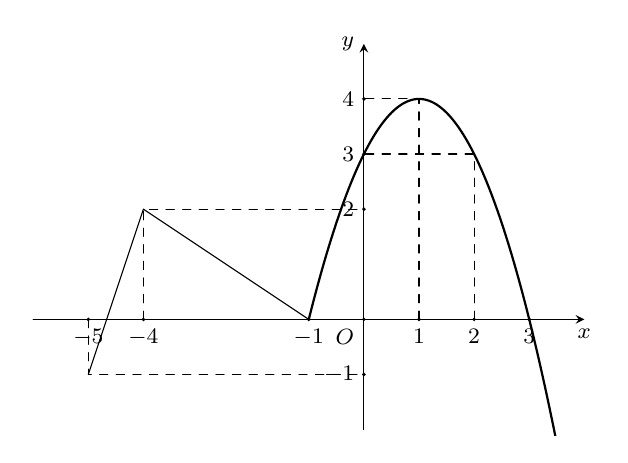
\begin{tikzpicture}[scale=0.7, font=\footnotesize, line join=round, line cap=round,>=stealth]
			%Gán số liệu.
			\def\xmin{-6};\def\ymin{-2};\def\xmax{4};\def\ymax{5};
			%Gán tọa độ.
			\coordinate (O) at (0,0);
			%Trục Oxy.
			\draw[->] (\xmin,0)--(\xmax,0) node[below]{$x$};
			\draw[->] (0,\ymin)--(0,\ymax) node[left]{$y$};
			\fill (O) node[below left]{$O$} circle(1pt);
			%Giới hạn đồ thị.
			\clip ({\xmin-0.1},{\ymin-0.1}) rectangle ({\xmax+0.1},{\ymax+0.1});
			\foreach \x in {-5,-4,-1,1,2,3}{
				\fill (\x,0) node[below]{$\x$} circle(1pt);
			}
			\foreach \y in {-1,2,3,4}{
				\fill (0,\y) node[left]{$\y$} circle(1pt);
			}
			\draw (-5,-1)--(-4,2)--(-1,0);
			\draw[thick,samples=100] plot[domain=-1:3.5](\x,{-(\x)^2+2*\x+3});
			\draw[dashed] (-5,0)|-(0,-1) (-4,0)|-(0,2) (1,0)|-(0,4) (2,0)|-(0,3);
		\end{tikzpicture}
	}
	\loigiai{
		Parabol $y=a x^2+b x+c$ qua các điểm $(2 ; 3)$, $(1 ; 4)$, $(0 ; 3)$, $(-1 ; 0)$, $(3 ; 0)$ nên xác định được $y=-x^2+2 x+3$, $\forall x \geq-1$ suy ra $f(x)=-\dfrac{x^3}{3}+x^2+3 x+C_1$.\\
		Mà $f(0)=0 \Rightarrow C_1=0$, $f(x)=-\dfrac{x^3}{3}+x^2+3 x$.\\
		Có $f(-1)=-\dfrac{5}{3}$, $ f(2)=\dfrac{22}{3}$.\quad $(1)$\\
		Đồ thị $f'(x)$ trên đoạn $[-4 ;-1]$ qua các điểm $(-4 ; 2)$, $(-1 ; 0)$.\\
		Nên $f'(x)=-\dfrac{2}{3}(x+1) \Rightarrow f(x)=-\dfrac{2}{3}\left(\dfrac{x^2}{2}+x\right)+C_2$.\\
		Mà $f(-1)=-\dfrac{5}{3} \Leftrightarrow C_2=-\dfrac{5}{3}+\dfrac{2}{3}\left(-\dfrac{1}{2}\right)=-2 \Rightarrow f(x)=-\dfrac{2}{3}\left(\dfrac{x^2}{2}+x\right)-2$, hay $f(-4)=-\dfrac{14}{3}$.\\
		Đồ thị $f'(x)$ trên đoạn $[-5 ;-4]$ qua các điểm $(-4 ; 2)$, $(-5 ;-1)$.\\
		Nên $f'(x)=3 x+14 \Rightarrow f(x)=\dfrac{3 x^2}{2}+14 x+C_3$.\\
		Mà $f(-4)=-\dfrac{14}{3} \Leftrightarrow \dfrac{3 \cdot(-4)^2}{2}+14 \cdot(-4)+C_3=-\dfrac{14}{3}$ suy ra $C_3=\dfrac{82}{3}$.\\
		Ta có $f(x)=\dfrac{3 x^2}{2}+14 x+\dfrac{82}{3} \Rightarrow f(-5)=-\dfrac{31}{6}$.\quad $(2)$\\
		Từ $(1)$ và $(2)$ ta được $2 f(-5)+3 f(2)=-\dfrac{31}{3}+22=\dfrac{35}{3}$.
	}
\end{ex}
\Closesolutionfile{ans}
% \indapan{10}{ans/ans-LC-2-C4B1CD3.1}